\documentclass{article}

% these packages let you do math
\usepackage{amsmath}
\usepackage{amssymb}

% we need these packages for fancy R tables
\usepackage{booktabs}
\usepackage{float}
\usepackage{colortbl}
\usepackage{xcolor}

% these packages play with the spacing/margins of the document. Uncomment the commands on lines 16 and 17 to see what they do.
\usepackage{a4wide}
\usepackage{setspace}
\usepackage{geometry}
\usepackage{parskip}
%\doublespacing
%\geometry{margin=1.5in}

% this package helps us with including images. Setting the graphics path makes it easier to refer to things in the \includegraphics command.
\usepackage{graphicx}
\graphicspath{ {../figures/} }

% make some hyperlinks using the \href command
\usepackage{hyperref}
\hypersetup{
    colorlinks=true,
    linkcolor=black,
    urlcolor=blue
}

% set the author, title, and date of the document. \maketitle adds it to the document.
\author{Xiaohan Wu}
\title{Paper on NLSY97 Data of Incarceration Status}
\date{Spring 2022}

\begin{document}
\maketitle

\section{Introduction}

This report describes patterns in monthly incarceration status by race and gender in the year 2002, using NLSY97 publicly available data. Before analyzing the dataset, the raw dataset was mined into a clean dataset with readable variables wanted.

The three variables to be analyzed are \texttt{race}, \texttt{gender}, and \texttt{total\_incarcerated}. The variable \texttt{race} includes \texttt{Black}, \texttt{Hispanic}, \texttt{Mixed Race}, and \texttt{Non-Black or Non-Hispanic}. The variable \texttt{total\_incarcerated} summarizes each respondent's monthly incarceration status in 2002, representing the respondent's total months of incarceration in 2022.

\section{Analysis}

\begin{figure}[H]
    \begin{center}
        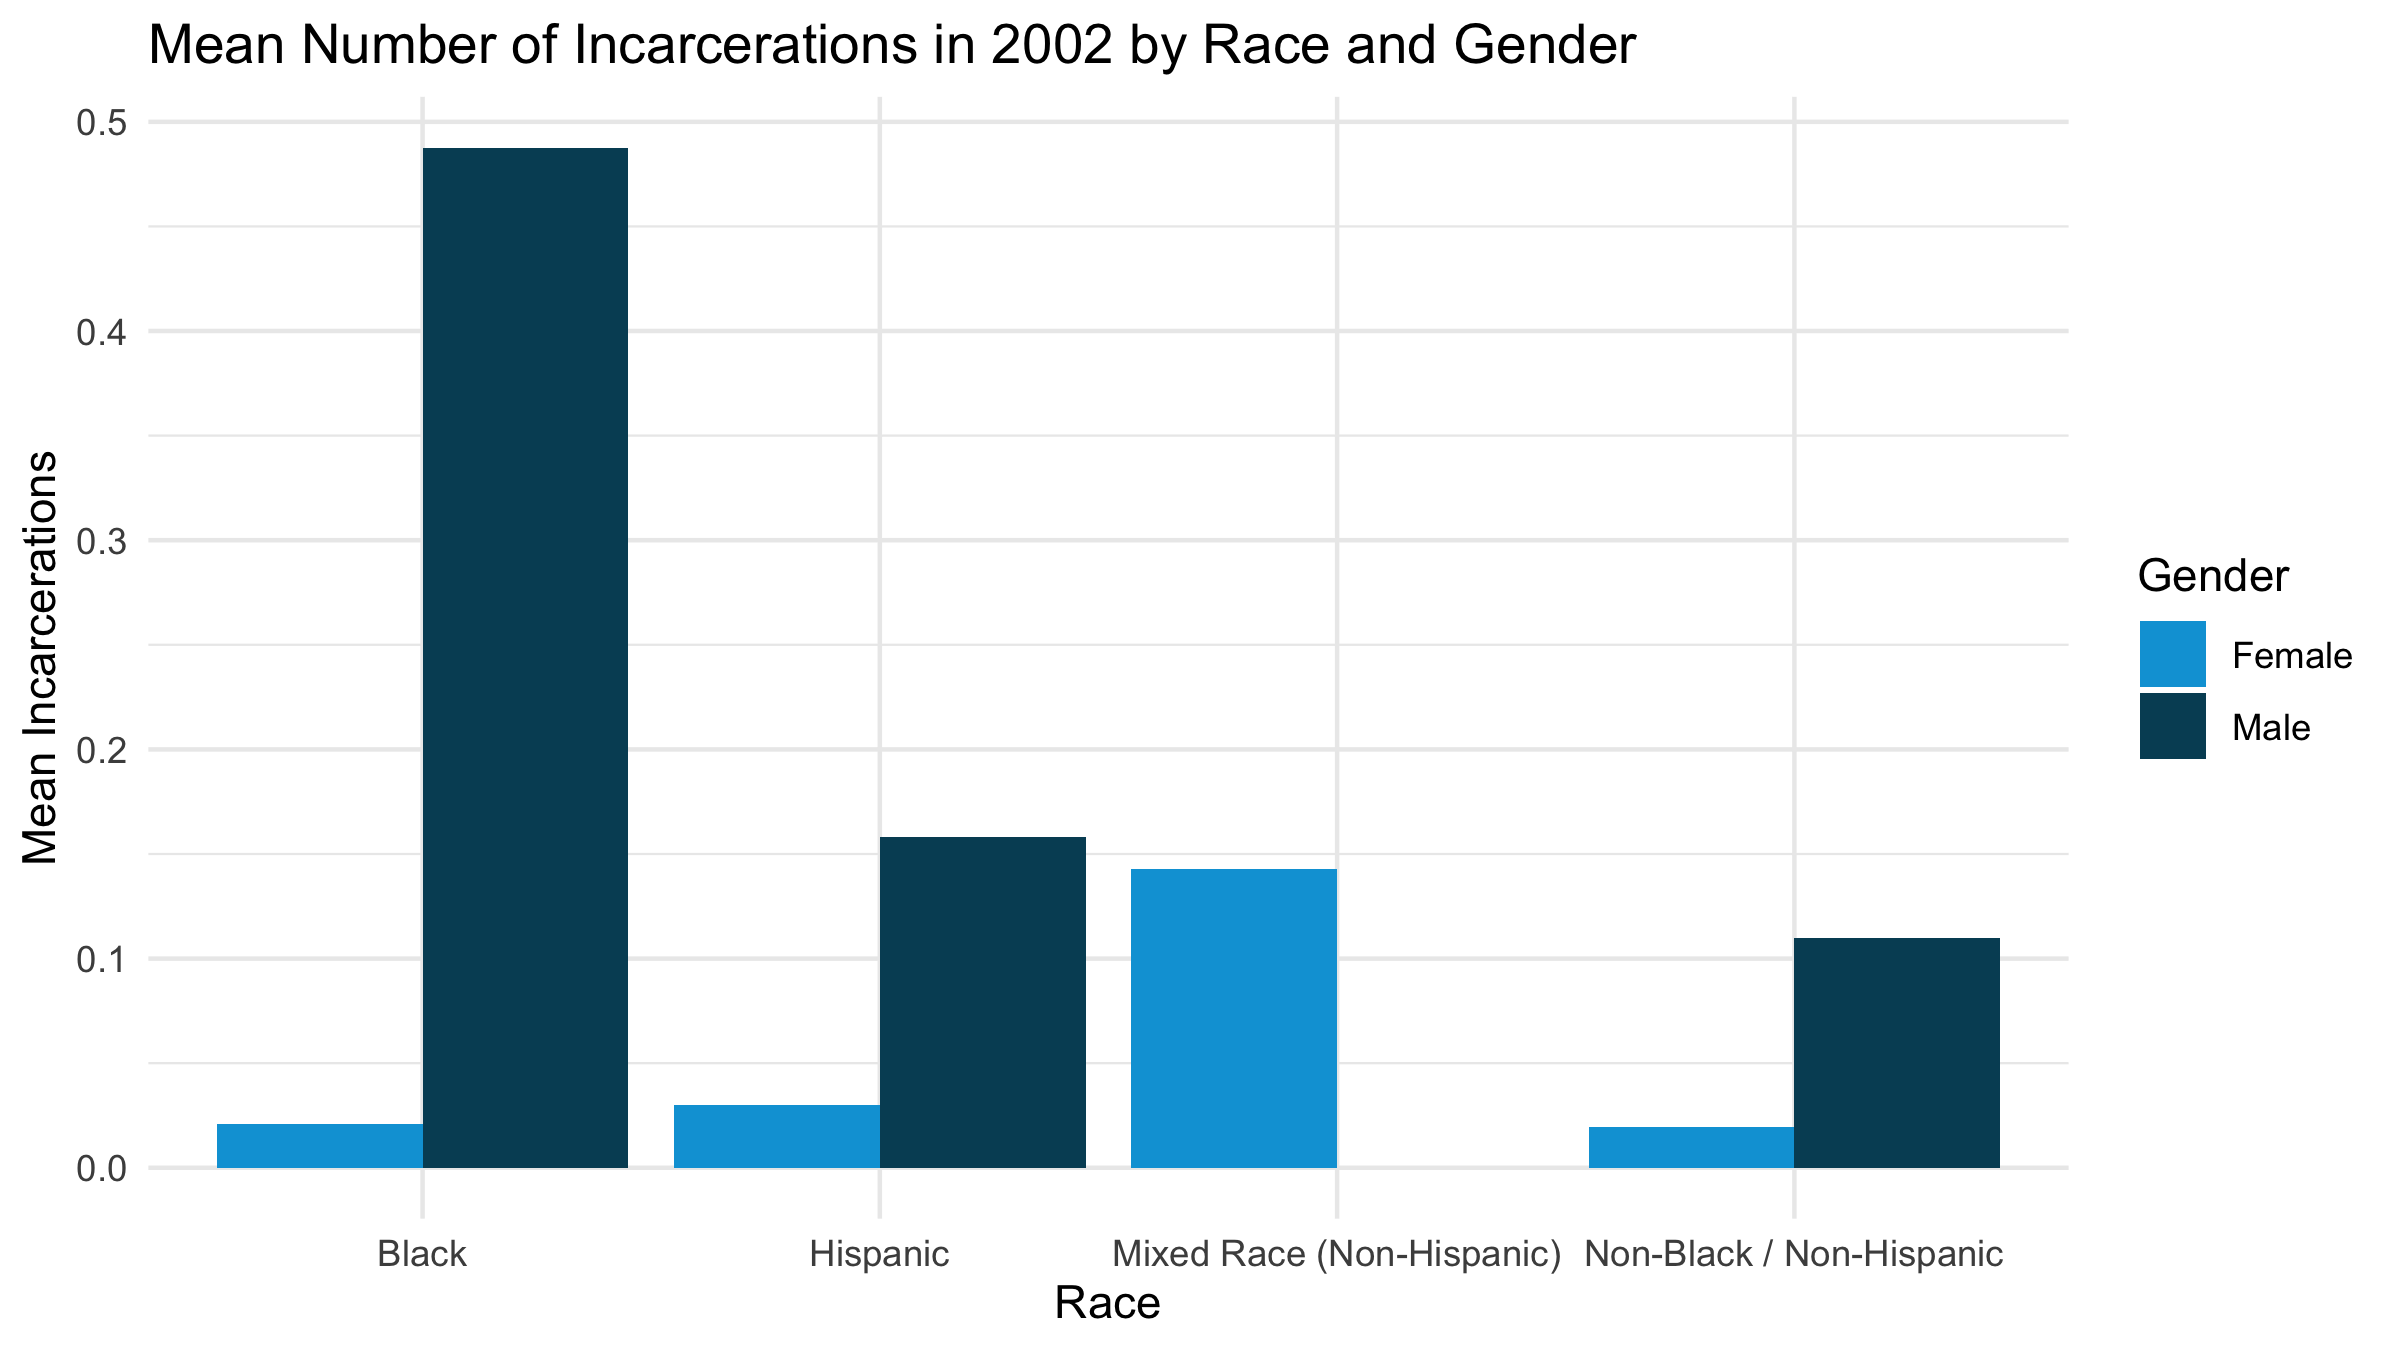
\includegraphics[width=.85\textwidth]{incarcerations_by_racegender}
    \end{center}
    \caption{Mean Number of Incarcerated Months in 2002 by Race and Gender}
    \label{fig:graph}
\end{figure}

\begin{table}[H]

\caption{\label{tab:tab:summarystats}Mean Number of incarcerated Months in 2002 by Race and Gender}
\centering
\begin{tabular}[t]{lrrrr}
\toprule
Gender & Black & Hispanic & Mixed Race Non Hispanic & Non Black Non Hispanic\\
\midrule
\cellcolor{gray!6}{Female} & \cellcolor{gray!6}{0.0211268} & \cellcolor{gray!6}{0.0298013} & \cellcolor{gray!6}{0.1428571} & \cellcolor{gray!6}{0.0193192}\\
Male & 0.4876712 & 0.1579509 & 0.0000000 & 0.1099476\\
\bottomrule
\end{tabular}
\end{table}


The Figure \ref{fig:graph} above is a barplot showing the mean number of incarcerated months in 2002 by \texttt{race} and \texttt{gender}, while Table 1 above is showing the detailed values.

For respondents whose variable \texttt{race} is \texttt{Black}, females' mean incarcerated month number is around 0.02, which is significantly lower than males' mean incarcerated month number (0.5). 

For respondents whose variable \texttt{race} is \texttt{Hispanic}, females' mean incarcerated month number is around 0.03, which is significantly lower than males' mean incarcerated month number (0.16). 

For respondents whose variable \texttt{race} is \texttt{Non-Black or Non-Hispanic}, females' mean incarcerated month number is around 0.02, which is significantly lower than males' mean incarcerated month number (0.11).

For the above three different races, it could be concluded that mainly the males would get much more incarcerations than females in the group of respondents.

However, for respondents whose variable \texttt{race} is \texttt{Mixed Race Non-Hispanic}, females' mean incarcerated month number is around 0.14, which is significantly higher than males' mean incarcerated month number (0). The result is quite unrealistic since the mean number of incarcerated months is unlikely to be 0 for males in any race category. A possible explanation would be that the gender for \texttt{Mixed Race Non-Hispanic} group is mistakenly recorded in the raw dataset. Further investigation and validation would be required and necessary.

\newpage


% Table created by stargazer v.5.2.2 by Marek Hlavac, Harvard University. E-mail: hlavac at fas.harvard.edu
% Date and time: Thu, Feb 17, 2022 - 02:37:03
\begin{table}[!htbp] \centering 
  \caption{Regression Output. Omitted category is Black Females.} 
  \label{tab:regression} 
\begin{tabular}{@{\extracolsep{5pt}}lc} 
\\[-1.8ex]\hline 
\hline \\[-1.8ex] 
 & \multicolumn{1}{c}{\textit{Dependent variable:}} \\ 
\cline{2-2} 
\\[-1.8ex] & Incarcerations in 2002 \\ 
\hline \\[-1.8ex] 
 Hispanic & $-$0.159$^{***}$ \\ 
  & (0.038) \\ 
  & \\ 
 Mixed Race (Non-Hispanic) & $-$0.174$^{**}$ \\ 
  & (0.083) \\ 
  & \\ 
 Non-Black / Non-Hispanic & $-$0.189$^{***}$ \\ 
  & (0.035) \\ 
  & \\ 
 Male & 0.194$^{***}$ \\ 
  & (0.022) \\ 
  & \\ 
 Constant & 0.155$^{***}$ \\ 
  & (0.026) \\ 
  & \\ 
\hline \\[-1.8ex] 
Observations & 8,621 \\ 
R$^{2}$ & 0.015 \\ 
Adjusted R$^{2}$ & 0.014 \\ 
Residual Std. Error & 1.019 (df = 8616) \\ 
F Statistic & 32.033$^{***}$ (df = 4; 8616) \\ 
\hline 
\hline \\[-1.8ex] 
\textit{Note:}  & \multicolumn{1}{r}{$^{*}$p$<$0.1; $^{**}$p$<$0.05; $^{***}$p$<$0.01} \\ 
\end{tabular} 
\end{table} 


The table above shows the regression output. The omitted category is Black Females. 

The regression result can be shown by the equation below:

\begin{equation*}
    total\_incarcerated = -0.159 Hispanic - 0.174 Mixed Race - .189 Non-Black or Non-Hispanic + 0.194 Male + 0.155
\end{equation*}

The coefficient of \texttt{Mixed Race} is sgnificant at 0.05 level, while all the other coefficients are significant at 0.01 level.

However, the regression's R-Squared value is extremely low (around 0,015), indicating the regression may not fit the dataset closely.

\section{The Next Steps}

First of all, the gender for \texttt{Mixed Race Non-Hispanic} group might be mistakenly recorded in the raw dataset. Further investigation and validation would be required and necessary.

The regression's R-Squared value is extremely low (around 0.015), indicating the regression may not fit the dataset closely. Further investigation should be performed.

\end{document}
